
%-------------------------------------------------------------------------------
%   PACKAGES AND OTHER DOCUMENT CONFIGURATIONS
%-------------------------------------------------------------------------------
\documentclass[12pt]{extbook} % Default font size and left-justified equations

%-------------------------------------------------------------------------------
%   Enable gray scale color theme in entire document
%-------------------------------------------------------------------------------
%\def\EnableGrayScale{1}

%-------------------------------------------------------------------------------
%   Widow and orphan lines
%-------------------------------------------------------------------------------
\clubpenalty=1000
\widowpenalty=1000 

%-------------------------------------------------------------------------------
%   ROOT PATH of tex source
%-------------------------------------------------------------------------------
\def \SourceRootPath{.}

%-------------------------------------------------------------------------------
%   DATOS: Title, subtitle, author, etc.
%-------------------------------------------------------------------------------
\input{\SourceRootPath/structure/head-macros/data-macros}

%-------------------------------------------------------------------------------
%   Color theme of book
%-------------------------------------------------------------------------------
\ifx\EnableGrayScale\undefined
    %%----------------------------------------------------------------------------------------
%	XCOLOR
%----------------------------------------------------------------------------------------
\usepackage[dvipsnames*,svgnames]{xcolor}
%% \colorlet{LightRubineRed}{RubineRed!70}
%% \colorlet{Mycolor1}{green!10!orange}
%% \definecolor{light-gray}{gray}{0.95}
%% \definecolor{Mycolor2}{HTML}{00F9DE}
%% \definecolor{orange}{rgb}{1,0.5,0}
%% \definecolor{DarkRed}{RGB}{98,32,6}
%% \definecolor{orange}{cmyk}{0,0.5,1,0}

% Colores básicos
\definecolor{ColorScheme1}{RGB}{48,48,48}
\definecolor{ColorScheme2}{RGB}{48,48,48}
\definecolor{ColorScheme3}{RGB}{64,64,64}
\definecolor{ColorScheme4}{RGB}{120,120,120}
\definecolor{ColorScheme5}{RGB}{240,240,240}
\definecolor{ColorScheme6}{RGB}{255,255,255}

% Default
\colorlet{colorDefault}{black} % Define the color used for highlighting throughout the book

% Part-chapter-title
\colorlet{colorTitlePage}{ColorScheme4}
\colorlet{colorPartPageBackground}{ColorScheme4}
\colorlet{colorPartText}{colorDefault}
\colorlet{colorChapter}{colorDefault}
\colorlet{colorSection}{colorDefault}
\colorlet{colorSectionFont}{colorDefault}
\colorlet{colorSubsection}{black}
\colorlet{colorSubsectionFont}{black}

% Boxs
\colorlet{colorAttention}{ColorScheme6}
\colorlet{colorAttentionFrame}{colorDefault}
\colorlet{colorBoxEquation}{ColorScheme5}
\colorlet{colorCitando}{ColorScheme5}
\colorlet{colorDefinition}{colorDefault}
\colorlet{colorElaboration}{ColorScheme3}
\colorlet{colorElaborationFrame}{colorDefault}
\colorlet{colorExample}{colorDefault}
\colorlet{colorExercise}{colorDefault}
\colorlet{colorFraseBox}{colorDefault}
\colorlet{colorInformationBox}{colorDefault}
\colorlet{colorLemma}{colorDefault}
\colorlet{colorNotation}{colorDefault}
\colorlet{colorTheorem}{colorDefault}
\colorlet{colorNote}{colorDefault!10}

% Otros
\colorlet{colormylink}{ColorScheme4}
\colorlet{colorIndex}{colorDefault}

% Init pages
\colorlet{colorPatrocinio}{ColorScheme3!10!white}


%----------------------------------------------------------------------------------------
%	COLOR
%----------------------------------------------------------------------------------------
\usepackage{color}


    %%----------------------------------------------------------------------------------------
%	XCOLOR
%----------------------------------------------------------------------------------------
\usepackage[dvipsnames*,svgnames]{xcolor}
%% \colorlet{LightRubineRed}{RubineRed!70}
%% \colorlet{Mycolor1}{green!10!orange}
%% \definecolor{light-gray}{gray}{0.95}
%% \definecolor{Mycolor2}{HTML}{00F9DE}
%% \definecolor{orange}{rgb}{1,0.5,0}
%% \definecolor{DarkRed}{RGB}{98,32,6}
%% \definecolor{orange}{cmyk}{0,0.5,1,0}

% Color theme
\definecolor{ColorScheme1}{RGB}{16,81,15}
\definecolor{ColorScheme2}{RGB}{217,168,91}
\definecolor{ColorScheme3}{RGB}{255,249,128}
\definecolor{ColorScheme4}{RGB}{105,46,60}
\definecolor{ColorScheme5}{RGB}{182,106,70}
\definecolor{ColorScheme6}{RGB}{240,240,240}

% Default
\colorlet{colorDefault}{ColorScheme1} % Define the color used for highlighting throughout the book

% Part-chapter-title
\colorlet{colorTitlePage}{ColorScheme4}
\colorlet{colorPartPageBackground}{ColorScheme5!50!black}
\colorlet{colorPartText}{colorDefault}
\colorlet{colorChapter}{colorDefault}
\colorlet{colorSection}{colorDefault}
\colorlet{colorSectionFont}{colorDefault}
\colorlet{colorSubsection}{black}
\colorlet{colorSubsectionFont}{black}

% Boxs
\colorlet{colorAttention}{ColorScheme3}
\colorlet{colorAttentionFrame}{colorDefault}
\colorlet{colorEquationBox}{ColorScheme6}
\colorlet{colorCitationBox}{ColorScheme6}
\colorlet{colorDefinition}{colorDefault}
\colorlet{colorElaboration}{colorDefault}
\colorlet{colorElaborationFrame}{colorDefault}
\colorlet{colorExample}{colorDefault}
\colorlet{colorExercise}{colorDefault}
\colorlet{colorFraseBox}{colorDefault}
\colorlet{colorInformationBox}{colorDefault}
\colorlet{colorLemma}{colorDefault}
\colorlet{colorNotation}{colorDefault}
\colorlet{colorTheorem}{colorDefault}
\colorlet{colorNote}{colorDefault!10}

% Otros
\colorlet{colormylink}{colorDefault}
\colorlet{colorIndex}{colorDefault}

% Init pages
\colorlet{colorPatrocinio}{ColorScheme6}


%----------------------------------------------------------------------------------------
%	COLOR
%----------------------------------------------------------------------------------------
\usepackage{color}


    %\input{\SourceRootPath/structure/color-scheme/tierra4}
    %%----------------------------------------------------------------------------------------
%	XCOLOR
%----------------------------------------------------------------------------------------
\usepackage[dvipsnames*,svgnames]{xcolor}
%% \colorlet{LightRubineRed}{RubineRed!70}
%% \colorlet{Mycolor1}{green!10!orange}
%% \definecolor{light-gray}{gray}{0.95}
%% \definecolor{Mycolor2}{HTML}{00F9DE}
%% \definecolor{orange}{rgb}{1,0.5,0}
%% \definecolor{DarkRed}{RGB}{98,32,6}
%% \definecolor{orange}{cmyk}{0,0.5,1,0}

% Color theme
\definecolor{ColorScheme1}{RGB}{22,75,89}
\definecolor{ColorScheme2}{RGB}{242,228,215}
\definecolor{ColorScheme3}{RGB}{255,184,118}
\definecolor{ColorScheme4}{RGB}{77,122,99}
\definecolor{ColorScheme5}{RGB}{120,120,120}
\definecolor{ColorScheme6}{RGB}{240,240,240}

% Default
\colorlet{colorDefault}{ColorScheme1} % Define the color used for highlighting throughout the book

% Part-chapter-title
\colorlet{colorTitlePage}{ColorScheme4}
\colorlet{colorPartPageBackground}{ColorScheme5!50!black}
\colorlet{colorPartText}{colorDefault}
\colorlet{colorChapter}{colorDefault}
\colorlet{colorSection}{colorDefault}
\colorlet{colorSectionFont}{colorDefault}
\colorlet{colorSubsection}{black}
\colorlet{colorSubsectionFont}{black}

% Boxs
\colorlet{colorAttention}{ColorScheme3}
\colorlet{colorAttentionFrame}{colorDefault}
\colorlet{colorEquationBox}{ColorScheme2!50}
\colorlet{colorCitationBox}{ColorScheme2!50}
\colorlet{colorDefinition}{ColorScheme4}
\colorlet{colorElaboration}{ColorScheme4}
\colorlet{colorElaborationFrame}{colorDefault}
\colorlet{colorExample}{ColorScheme4}
\colorlet{colorExercise}{ColorScheme4}
\colorlet{colorPhraseBox}{ColorScheme2}
\colorlet{colorInformationBox}{ColorScheme4}
\colorlet{colorLemma}{ColorScheme4}
\colorlet{colorNotation}{ColorScheme4}
\colorlet{colorTheorem}{ColorScheme4}
\colorlet{colorNote}{ColorScheme4!10}

% Otros
\colorlet{colormylink}{ColorScheme4}
\colorlet{colorIndex}{colorDefault}

% Init pages
\colorlet{colorPatrocinio}{ColorScheme2!50}


%----------------------------------------------------------------------------------------
%	COLOR
%----------------------------------------------------------------------------------------
\usepackage{color}


    %\input{\SourceRootPath/structure/color-scheme/manta2}
    %----------------------------------------------------------------------------------------
%	XCOLOR
%----------------------------------------------------------------------------------------

%% \colorlet{LightRubineRed}{RubineRed!70}
%% \colorlet{Mycolor1}{green!10!orange}
%% \definecolor{light-gray}{gray}{0.95}
%% \definecolor{Mycolor2}{HTML}{00F9DE}
%% \definecolor{orange}{rgb}{1,0.5,0}
%% \definecolor{DarkRed}{RGB}{98,32,6}
%% \definecolor{orange}{cmyk}{0,0.5,1,0}

% Color theme
\definecolor{ColorScheme1}{RGB}{74,84,174}%azul
\definecolor{ColorScheme2}{RGB}{21,146,129}%verde
\definecolor{ColorScheme3}{RGB}{249,247,211}%amarelo
\definecolor{ColorScheme4}{RGB}{190,59,47}%rojo
\definecolor{ColorScheme5}{RGB}{186,213,133}%verde low
\definecolor{ColorScheme6}{RGB}{95,125,182}%azul low

% Default
\colorlet{colorDefault}{ColorScheme6} % Define the color used for highlighting throughout the book

% Part-chapter-title
\colorlet{colorTitlePage}{ColorScheme4}
\colorlet{colorPartPageBackground}{ColorScheme5!50!black}
\colorlet{colorPartText}{colorDefault}
\colorlet{colorChapter}{colorDefault}
\colorlet{colorSection}{colorDefault}
\colorlet{colorSectionFont}{colorDefault}
\colorlet{colorSubsection}{ColorScheme4}
\colorlet{colorSubsectionFont}{ColorScheme4}

% Boxs
\colorlet{colorAttention}{ColorScheme3}
\colorlet{colorAttentionFrame}{colorDefault}
\colorlet{colorEquationBox}{ColorScheme6!20}
\colorlet{colorCitationBox}{ColorScheme6!20}
\colorlet{colorDefinition}{ColorScheme4}
\colorlet{colorElaboration}{ColorScheme4}
\colorlet{colorElaborationFrame}{colorDefault}
\colorlet{colorExample}{ColorScheme2}
\colorlet{colorExercise}{ColorScheme6}
\colorlet{colorPhraseBox}{ColorScheme6}
\colorlet{colorInformationBox}{ColorScheme4}
\colorlet{colorLemma}{ColorScheme4}
\colorlet{colorNotation}{ColorScheme6}
\colorlet{colorTheorem}{colorDefault}
\colorlet{colorNote}{ColorScheme4!10}

% Otros
\colorlet{colormylink}{ColorScheme4}
\colorlet{colorIndex}{colorDefault}

% Init pages
\colorlet{colorPatrocinio}{ColorScheme3}


%----------------------------------------------------------------------------------------
%	COLOR
%----------------------------------------------------------------------------------------
\usepackage{color}


\else
    %----------------------------------------------------------------------------------------
%	XCOLOR
%----------------------------------------------------------------------------------------
\usepackage[dvipsnames*,svgnames]{xcolor}
%% \colorlet{LightRubineRed}{RubineRed!70}
%% \colorlet{Mycolor1}{green!10!orange}
%% \definecolor{light-gray}{gray}{0.95}
%% \definecolor{Mycolor2}{HTML}{00F9DE}
%% \definecolor{orange}{rgb}{1,0.5,0}
%% \definecolor{DarkRed}{RGB}{98,32,6}
%% \definecolor{orange}{cmyk}{0,0.5,1,0}

% Colores básicos
\definecolor{ColorScheme1}{RGB}{48,48,48}
\definecolor{ColorScheme2}{RGB}{48,48,48}
\definecolor{ColorScheme3}{RGB}{64,64,64}
\definecolor{ColorScheme4}{RGB}{120,120,120}
\definecolor{ColorScheme5}{RGB}{240,240,240}
\definecolor{ColorScheme6}{RGB}{255,255,255}

% Default
\colorlet{colorDefault}{black} % Define the color used for highlighting throughout the book

% Part-chapter-title
\colorlet{colorTitlePage}{ColorScheme4}
\colorlet{colorPartPageBackground}{ColorScheme4}
\colorlet{colorPartText}{colorDefault}
\colorlet{colorChapter}{colorDefault}
\colorlet{colorSection}{colorDefault}
\colorlet{colorSectionFont}{colorDefault}
\colorlet{colorSubsection}{black}
\colorlet{colorSubsectionFont}{black}

% Boxs
\colorlet{colorAttention}{ColorScheme6}
\colorlet{colorAttentionFrame}{colorDefault}
\colorlet{colorBoxEquation}{ColorScheme5}
\colorlet{colorCitando}{ColorScheme5}
\colorlet{colorDefinition}{colorDefault}
\colorlet{colorElaboration}{ColorScheme3}
\colorlet{colorElaborationFrame}{colorDefault}
\colorlet{colorExample}{colorDefault}
\colorlet{colorExercise}{colorDefault}
\colorlet{colorFraseBox}{colorDefault}
\colorlet{colorInformationBox}{colorDefault}
\colorlet{colorLemma}{colorDefault}
\colorlet{colorNotation}{colorDefault}
\colorlet{colorTheorem}{colorDefault}
\colorlet{colorNote}{colorDefault!10}

% Otros
\colorlet{colormylink}{ColorScheme4}
\colorlet{colorIndex}{colorDefault}

% Init pages
\colorlet{colorPatrocinio}{ColorScheme3!10!white}


%----------------------------------------------------------------------------------------
%	COLOR
%----------------------------------------------------------------------------------------
\usepackage{color}


\fi

%-------------------------------------------------------------------------------
%   All used packages: comment,lipsum, calc, morewrites, booktabs, etc.
%-------------------------------------------------------------------------------

%----------------------------------------------------------------------------------------
%	XCOLOR
%----------------------------------------------------------------------------------------
\usepackage[dvipsnames*,svgnames,table]{xcolor}

%----------------------------------------------------------------------------------------
%   
%----------------------------------------------------------------------------------------
\usepackage{comment} %
\usepackage{lipsum} % Inserts dummy text
\usepackage{calc}   % For simpler calculation - used for spacing the index letter headings correctly
\usepackage{morewrites}%%! No room for a new \write.
\usepackage{booktabs} %% Required for nicer horizontal rules in tables \toprule \midrule \bottomrule
\usepackage{etoolbox} %% necesario para ifdefstring
\usepackage{fancyvrb}
\usepackage{lmodern}  % The lmodern package was used just to have access to a 80pt font size.

%----------------------------------------------------------------------------------------
%	ACENTOS
%----------------------------------------------------------------------------------------
\usepackage[utf8]{inputenc} % Required for including letters with accents
\usepackage[T1]{fontenc} % Use 8-bit encoding that has 256 glyphs

\usepackage[brazil]{babel}
%\usepackage[english]{babel} % English language/hyphenation

%----------------------------------------------------------------------------------------
%	FONTS
%----------------------------------------------------------------------------------------
\usepackage{avant} % Use the Avantgarde font for headings
%\usepackage{times} % Use the Times font for headings
\usepackage{mathptmx} % Use the Adobe Times Roman as the default text font together with math symbols from the Sym­bol, Chancery and Com­puter Modern fonts
\usepackage{microtype}% The microtype package was used to use \textls to space out the letters in "Chapter". % Slightly tweak font spacing for aesthetics



%----------------------------------------------------------------------------------------
%	PAGE HEADERS
%----------------------------------------------------------------------------------------

\usepackage{fancyhdr} % Required for header and footer configuration
\pagestyle{fancy}


%----------------------------------------------------------------------------------------
% Para 
% \begin{inparaenum}
% \item
% \end{inparaenum}
% parecido a timeze pero horizontal 
%----------------------------------------------------------------------------------------
\usepackage{paralist}
\usepackage{enumitem} % Customize lists % en ese orden primero paralist
\setlist{nolistsep} % Reduce spacing between bullet points and numbered lists


%----------------------------------------------------------------------------------------
%	VARIOUS REQUIRED PACKAGES AND CONFIGURATIONS
%----------------------------------------------------------------------------------------

\usepackage[%
paperwidth=\BookPaperWidth,
paperheight=\BookPaperHeight, 
top=\BookMarginTop,%
bottom=\BookMarginBottom,%
left=\BookMarginLeft,%
right=\BookMarginRight,%
headsep=10pt]{geometry} % Page margins

%----------------------------------------------------------------------------------------
% Graficos
%----------------------------------------------------------------------------------------
\usepackage{graphicx} % Required for including pictures
\usepackage{float}% para ter [H]
\graphicspath{{pictures/}} % Specifies the directory where pictures are stored
%\graphicspath{{pictures/}{pictures/social-network/}{pictures/chapter_head/}{pictures/rule-separator/}}
\ifdefined \EnableGrayScale
    \usepackage[GRAY]{epspdfconversion}
\fi

\usepackage{eso-pic}%%This package makes it easy to add some picture commands (background) to every page at ab-solute positions

%----------------------------------------------------------------------------------------
% Par diferentes modelos de caption.
%----------------------------------------------------------------------------------------
\usepackage{caption}
\usepackage{subcaption}
\usepackage{wrapfig}

%----------------------------------------------------------------------------------------
% ROTATION FIGURE
%----------------------------------------------------------------------------------------
% For rotating figures, tables, etc.
%  including their captions
% \begin{sidewaysfigure}[ht]
% \end{sidewaysfigure}
\usepackage[figuresleft]{rotating}


%----------------------------------------------------------------------------------------
%	Footnote
%----------------------------------------------------------------------------------------
\usepackage{scrextend} %multiple reference

%----------------------------------------------------------------------------------------
%  footnote font size
%----------------------------------------------------------------------------------------
\renewcommand{\footnotesize}{\small}

%----------------------------------------------------------------------------------------
% Page counter
%----------------------------------------------------------------------------------------
\usepackage{lastpage}

%----------------------------------------------------------------------------------------
% GLOSSARIO
%----------------------------------------------------------------------------------------
\usepackage{nomencl}

%----------------------------------------------------------------------------------------
% Para \singlespacing 
%----------------------------------------------------------------------------------------
\usepackage{setspace}

%----------------------------------------------------------------------------------------
% MUSICAL NOTATION
%----------------------------------------------------------------------------------------
\usepackage[generate,ps2eps]{abc}%%sudo apt-get install abcm2ps
\usepackage[nointegrals]{wasysym}
\usepackage{harmony} % http://linorg.usp.br/CTAN/macros/latex/contrib/harmony/harmony.pdf
\usepackage{leadsheets}%%https://ctan.math.illinois.edu/macros/latex/contrib/leadsheets/leadsheets_en.pdf


%----------------------------------------------------------------------------------------
% QR CODE
%----------------------------------------------------------------------------------------
%\usepackage{qrcode}

%----------------------------------------------------------------------------------------
%	DEFINITION OF THEOREM BOXES
%----------------------------------------------------------------------------------------
\usepackage{amsmath,amsfonts,amssymb,amsthm} % For math equations, theorems, symbols, etc

%----------------------------------------------------------------------------------------
% TIKZ
%----------------------------------------------------------------------------------------
\usepackage{tikz} % Required for drawing custom shapes
\usetikzlibrary{decorations.pathmorphing}

%----------------------------------------------------------------------------------------
% BOX - TCOLORBOX
%----------------------------------------------------------------------------------------
\usepackage[most,many]{tcolorbox}
\tcbuselibrary{skins}

%----------------------------------------------------------------------------------------
% Grafico circulo satelites
%----------------------------------------------------------------------------------------
\usepackage{smartdiagram}

%----------------------------------------------------------------------------------------
% Hacer indices
%----------------------------------------------------------------------------------------
\usepackage{makeidx} % Required to make an index
\makeindex % Tells LaTeX to create the files required for indexing


%----------------------------------------------------------------------------------------
%	BIBLIOGRAPHY AND INDEX
%----------------------------------------------------------------------------------------
\usepackage[ style=alphabetic,
             citestyle=alphabetic,
             sorting=none,
             sortcites=true,
             autopunct=true,
             babel=hyphen,
             hyperref=true,
             abbreviate=false,
             backref=true,
             backend=biber]{biblatex}
\addbibresource{bibliography/bibliography.bib} % BibTeX bibliography file
\defbibheading{bibempty}{}
%\renewcommand*{\bibfont}{\footnotesize}%%fontsize 

%----------------------------------------------------------------------------------------
%  BIBLIGRAHY font size
%----------------------------------------------------------------------------------------
\renewcommand*{\bibfont}{\footnotesize}

%----------------------------------------------------------------------------------------
% SIMILAR A ITEMIZE OU ENUMERATE
%----------------------------------------------------------------------------------------
\usepackage{tasks}

\settasks{
style=itemize, 
column-sep=5mm,
%label-format={\color{green!70!black}\large\bfseries},  
label-align=left, 
%label-offset={1mm}, 
%label-width={3mm}, 
%item-indent={1mm},
%item-format={\scshape\small}, 
%after-item-skip=1mm, 
%after-skip={10mm}
}


%----------------------------------------------------------------------------------------
% TABLE BREAKING
%----------------------------------------------------------------------------------------
\usepackage{longtable}

%----------------------------------------------------------------------------------------
% TABLE MULTIROW
%----------------------------------------------------------------------------------------
\usepackage{multirow}


%----------------------------------------------------------------------------------------
%	CONTROL PART, CHAPTER AND SECTION TITLE
%----------------------------------------------------------------------------------------
\usepackage[explicit]{titlesec} % necesario para titleformat

%----------------------------------------------------------------------------------------
%	MAIN TABLE OF CONTENTS
%----------------------------------------------------------------------------------------
\usepackage{titletoc} % Required for manipulating the table of contents

%----------------------------------------------------------------------------------------
%% OBLIGATORIAMENTE DEBE IR DESPUES DE TITLESEC Y TITLETOC
%----------------------------------------------------------------------------------------
%	HYPERLINKS IN THE DOCUMENTS 
%----------------------------------------------------------------------------------------
\usepackage{hyperref}
%% \usepackage{hyperxmp} %% da erro nao ativar- pdfcontactemail
\hypersetup{
	hidelinks,
	backref=true,
	pagebackref=true,
	hyperindex=true,
	colorlinks=true,
    citecolor=colorLink,    % color of citations
	linkcolor=black,          % color of internal links (change box color with linkbordercolor)
	%pdftoolbar=true,         % show Acrobat’s toolbar?
	%pdfmenubar=true,         % show Acrobat’s menu?
	%pdffitwindow=false,      % window fit to page when opened
	%pdfstartview={FitH},     % fits the width of the page to the window
	breaklinks=true,
	urlcolor= colorLink,
	bookmarks=true,
	bookmarksopen=false,
	pdftitle={\BookTitle - \BookSubTitle},
	pdfauthor={\BookAuthor},
	pdfsubject={\BookTitle - \BookSubTitle},
	pdfkeywords={\BookKeyWordA, \BookKeyWordB, \BookKeyWordC},
	%pdfcontactemail={\ImprimirRawEmail},
	%pdfcopyright={Creative Commons Atribuição - Não Comercial - Sem Derivações 4.0 Internacional},
	%baseurl={\BookLinkHomePage}
}


\usepackage{xurl} %melhor quebra de linha referencias

\usepackage{bookmark}%% precisa usepackage hyperref
\bookmarksetup{
open,
numbered,
addtohook={%
\ifnum\bookmarkget{level}=0 % chapter
\bookmarksetup{bold}%
\fi
\ifnum\bookmarkget{level}=-1 % part
\bookmarksetup{color=colorLink,bold}%
\fi
}
}


% Adiciona o diretório "paquetes" ao caminho de busca
\makeatletter
\def\input@path{{./packages}}
\makeatother

 %

%-------------------------------------------------------------------------------
%   Rules macros: \HRule{2pt}, \HTextRule{Text}
%-------------------------------------------------------------------------------
\usepackage{packages/separator-rule} %

%-------------------------------------------------------------------------------
%   Generic macros: \fprshowfont, etc.
%-------------------------------------------------------------------------------

%-------------------------------------------------------------------------------
% Font information
%-------------------------------------------------------------------------------
%   \fprshowfont
%-------------------------------------------------------------------------------
\makeatletter
\newcommand{\fprshowfont}{codifica\c{c}\~ao: \f@encoding{},
  familia: \f@family{},
  serie: \f@series{},
  %shape: \f@shape{},
  e tamanho: \f@size{} pt
}
\makeatother

%-------------------------------------------------------------------------------
% Formato de cada entrada da tabla de contenidos dos enviroments
%-------------------------------------------------------------------------------
%   \TocEntryEnvTextFormat
%-------------------------------------------------------------------------------
\newcommand{\TocEntryEnvTextFormat}{}
%\newcommand{\TocEntryEnvTextFormat}{\addvspace{3pt}\sffamily\bfseries}



 %


%-------------------------------------------------------------------------------
%   Math Macros: \FuncOf{f}{x}, \MinOf{x}{f(x)}, \ArgMin{x}{f(x)}, etc.
%-------------------------------------------------------------------------------
\usepackage{packages/math-macros} %

%-------------------------------------------------------------------------------
%   Configura el paquete titlesec 
%-------------------------------------------------------------------------------

\usetikzlibrary{shapes,shadows,calc}
\usetikzlibrary{positioning,calc}



\newcommand\SecTitle[5]{%
\begin{tikzpicture}

    \node (A) [rectangle,minimum width=\textwidth, minimum height=1cm,color=white,fill=colorsystemdefault, text width=\textwidth-3cm,align=left] {\hspace{1.5cm}\parbox{\textwidth}{\huge\textbf{\textsf{#4}}}};
    \fill[fill=colorsystemdefault!80] (A.north west) -- ($(A.north west)+(1.5cm,0)$) -- ($0.5*(A.north west)-0.5*(A.north west)-(0.5*\textwidth-2.5cm,0)$)--($(A.south west)+(1.5cm,0)$)--(A.south west);
    \node [color=white](A.north west) at ($0.5*(A.north west)-0.5*(A.north west)-(0.5*\textwidth-1cm,0)$) {\Huge\textbf{\textsf{#5}}};

\end{tikzpicture}

}

\titleformat{\section}
{\normalfont}{}{0em}
{\SecTitle{east}{west}{0\paperwidth}{#1}{\thesection}}

\titleformat{name=\section,numberless}
{\normalfont}{}{0em}
{\SecTitle{east}{west}{0\paperwidth}{#1}{~}}

    % titleformat de part [config-1 ..config-4]
\usepackage[
BanerColor=colorChapter,
BanerInner=0.6cm,
TitleColor=white,
TitleFontsize=30,
PreTitleColor=colorChapter,
PreTitleFontsize=16,
PreTitleNumberFontsize=30,
PreTitleNumberColor=white,
PreTitleNumberBackgroundColor=colorChapter,
PreTitleNumberWidth=1.7cm,
PreTitleNumberHeight=1.7cm,
PreTitleNumberYOffset=0.4cm,
AfterSpace=-25pt
]
{chapter-format-formalbar}

 % titleformat de chapter [config-1 ..config-5]

\titlespacing*{\part}{-10pt}{120pt}{-80pt}%pbk
\titleformat{\part}[frame]{\Huge\filcenter\bfseries}{ \normalfont\bf\fontsize{60pt}{0pt}\selectfont \raisebox{1.7cm}{ Part\fontfamily{put}\fontseries{b}\fontsize{60pt}{0pt}\selectfont \hspace{.2em}\thepart} }{30pt}{#1}[\filright]

 % titleformat de section [config-1 ..config-4]

\titlespacing*{\part}{-10pt}{120pt}{-80pt}%pbk
\titleformat{\part}[frame]{\Huge\filcenter\bfseries}{ \normalfont\bf\fontsize{60pt}{0pt}\selectfont \raisebox{1.7cm}{ Part\fontfamily{put}\fontseries{b}\fontsize{60pt}{0pt}\selectfont \hspace{.2em}\thepart} }{30pt}{#1}[\filright]

 % titleformat de subsection [config-1]

%-------------------------------------------------------------------------------
%   Configura header and footer 
%-------------------------------------------------------------------------------

\titlespacing*{\part}{-10pt}{120pt}{-80pt}%pbk
\titleformat{\part}[frame]{\Huge\filcenter\bfseries}{ \normalfont\bf\fontsize{60pt}{0pt}\selectfont \raisebox{1.7cm}{ Part\fontfamily{put}\fontseries{b}\fontsize{60pt}{0pt}\selectfont \hspace{.2em}\thepart} }{30pt}{#1}[\filright]

 % format [config-1]

%-------------------------------------------------------------------------------
%   Box enviroments
%-------------------------------------------------------------------------------
%----------------------------------------------------------------------------------------
% HIGHLIGHTBOX BOX
%----------------------------------------------------------------------------------------
% \begin{highlightbox}
%   text
% \end{highlightbox}

\usepackage{packages/env-highlightbox-zigzag}

\SetEnvHighlightBoxZigzagThickness{1pt}
\SetEnvHighlightBoxZigzagAmplitude{3pt}

\SetEnvHighlightBoxZigzagFrameColor{gray!60}
\SetEnvHighlightBoxZigzagBackColor{gray!10}

\SetEnvHighlightBoxZigzagBeforeSpace{1ex}
\SetEnvHighlightBoxZigzagAfterSpace{1ex}

\SetEnvHighlightBoxZigzagLeftPadding{2ex}
\SetEnvHighlightBoxZigzagRightPadding{2ex}
\SetEnvHighlightBoxZigzagTopPadding{2ex}
\SetEnvHighlightBoxZigzagBottomPadding{2ex}

 % format [tcolorbox-1]
%----------------------------------------------------------------------------------------
% ATTENTION MESSAGE BOX
%----------------------------------------------------------------------------------------
% \begin{attentionbox}
%   text
% \end{attentionbox}

\usepackage{env-highlight-foldedcorner}

\NewEnvBoxFoldedCornerGlobal[
BackColor=colorAttention!50,
FrameColor=colorAttention!50!black,
FoldColor=colorAttention!20!black,
ThicknessLength=1pt,
LeftSkipLength=0cm,
RightSkipLength=0cm,
ArcLength=3mm,
LeftRuleLength=10mm,
LeftRuleColor=colorAttention!50,
ImageObject={
\includegraphics[width=8mm]{icons/attention1.eps}},
BeforeSpaceLength=4pt,
AfterSpaceLength=4pt,
QedSymbol={},
ShadowColor=gray,
LeftPaddingLength=0ex,
RightPaddingLength=1ex,
TopPaddingLength=1.5ex,
BottomPaddingLength=1.5ex,
Breakable=true
]{attentionbox}

\begin{comment}
%% Define before space
\newcommand{\EnvAttentionBoxBeforeSpace}{2ex}
\newcommand{\SetEnvAttentionBoxBeforeSpace}[1]{\renewcommand{\EnvAttentionBoxBeforeSpace}{#1}}%

%% Define after space
\newcommand{\EnvAttentionBoxAfterSpace}{2ex}
\newcommand{\SetEnvAttentionBoxAfterSpace}[1]{\renewcommand{\EnvAttentionBoxAfterSpace}{#1}}%


\newtcolorbox{attentionbox}[1][]{enhanced,
  before skip=\EnvAttentionBoxBeforeSpace,after skip=\EnvAttentionBoxAfterSpace,
  boxrule=0.4pt,left=12mm,right=2mm,top=1mm,bottom=1mm,
  colback=colorAttention!50,
  colframe=colorAttention!20!black,
  sharp corners,rounded corners=southeast,arc is angular,arc=3mm,
  underlay={%
    \path[fill=colorAttentionFrame!20!black] ([yshift=3mm]interior.south east)--++(-0.4,-0.1)--++(0.1,-0.2);
    \path[draw=colorAttentionFrame,shorten <=-0.05mm,shorten >=-0.05mm] ([yshift=3mm]interior.south east)--++(-0.4,-0.1)--++(0.1,-0.2);
    \path[fill=colorAttention!50,draw=none] (interior.south west) rectangle node[white]{
\includegraphics[width=8mm]{icons/attention1.eps}} ([xshift=14mm]interior.north west);
    },
  drop fuzzy shadow,#1}
\end{comment}

 % format [tcolorbox-1 ... tcolorbox-3]
%----------------------------------------------------------------------------------------
% ATTENTION MESSAGE BOX
%----------------------------------------------------------------------------------------
% \begin{attentionbox}
%   text
% \end{attentionbox}

\usepackage{env-highlight-foldedcorner}

\NewEnvBoxFoldedCornerGlobal[
BackColor=colorAttention!50,
FrameColor=colorAttention!50!black,
FoldColor=colorAttention!20!black,
ThicknessLength=1pt,
LeftSkipLength=0cm,
RightSkipLength=0cm,
ArcLength=3mm,
LeftRuleLength=10mm,
LeftRuleColor=colorAttention!50,
ImageObject={
\includegraphics[width=8mm]{icons/attention1.eps}},
BeforeSpaceLength=4pt,
AfterSpaceLength=4pt,
QedSymbol={},
ShadowColor=gray,
LeftPaddingLength=0ex,
RightPaddingLength=1ex,
TopPaddingLength=1.5ex,
BottomPaddingLength=1.5ex,
Breakable=true
]{attentionbox}

\begin{comment}
%% Define before space
\newcommand{\EnvAttentionBoxBeforeSpace}{2ex}
\newcommand{\SetEnvAttentionBoxBeforeSpace}[1]{\renewcommand{\EnvAttentionBoxBeforeSpace}{#1}}%

%% Define after space
\newcommand{\EnvAttentionBoxAfterSpace}{2ex}
\newcommand{\SetEnvAttentionBoxAfterSpace}[1]{\renewcommand{\EnvAttentionBoxAfterSpace}{#1}}%


\newtcolorbox{attentionbox}[1][]{enhanced,
  before skip=\EnvAttentionBoxBeforeSpace,after skip=\EnvAttentionBoxAfterSpace,
  boxrule=0.4pt,left=12mm,right=2mm,top=1mm,bottom=1mm,
  colback=colorAttention!50,
  colframe=colorAttention!20!black,
  sharp corners,rounded corners=southeast,arc is angular,arc=3mm,
  underlay={%
    \path[fill=colorAttentionFrame!20!black] ([yshift=3mm]interior.south east)--++(-0.4,-0.1)--++(0.1,-0.2);
    \path[draw=colorAttentionFrame,shorten <=-0.05mm,shorten >=-0.05mm] ([yshift=3mm]interior.south east)--++(-0.4,-0.1)--++(0.1,-0.2);
    \path[fill=colorAttention!50,draw=none] (interior.south west) rectangle node[white]{
\includegraphics[width=8mm]{icons/attention1.eps}} ([xshift=14mm]interior.north west);
    },
  drop fuzzy shadow,#1}
\end{comment}

 % format [tcolorbox-1 ... tcolorbox-3]
%----------------------------------------------------------------------------------------
% HIGHLIGHTBOX BOX
%----------------------------------------------------------------------------------------
% \begin{highlightbox}
%   text
% \end{highlightbox}

\usepackage{packages/env-highlightbox-zigzag}

\SetEnvHighlightBoxZigzagThickness{1pt}
\SetEnvHighlightBoxZigzagAmplitude{3pt}

\SetEnvHighlightBoxZigzagFrameColor{gray!60}
\SetEnvHighlightBoxZigzagBackColor{gray!10}

\SetEnvHighlightBoxZigzagBeforeSpace{1ex}
\SetEnvHighlightBoxZigzagAfterSpace{1ex}

\SetEnvHighlightBoxZigzagLeftPadding{2ex}
\SetEnvHighlightBoxZigzagRightPadding{2ex}
\SetEnvHighlightBoxZigzagTopPadding{2ex}
\SetEnvHighlightBoxZigzagBottomPadding{2ex}

 

%-------------------------------------------------------------------------------
%   Theorems enviroments 
%-------------------------------------------------------------------------------
%----------------------------------------------------------------------------------------
% HIGHLIGHTBOX BOX
%----------------------------------------------------------------------------------------
% \begin{highlightbox}
%   text
% \end{highlightbox}

\usepackage{packages/env-highlightbox-zigzag}

\SetEnvHighlightBoxZigzagThickness{1pt}
\SetEnvHighlightBoxZigzagAmplitude{3pt}

\SetEnvHighlightBoxZigzagFrameColor{gray!60}
\SetEnvHighlightBoxZigzagBackColor{gray!10}

\SetEnvHighlightBoxZigzagBeforeSpace{1ex}
\SetEnvHighlightBoxZigzagAfterSpace{1ex}

\SetEnvHighlightBoxZigzagLeftPadding{2ex}
\SetEnvHighlightBoxZigzagRightPadding{2ex}
\SetEnvHighlightBoxZigzagTopPadding{2ex}
\SetEnvHighlightBoxZigzagBottomPadding{2ex}


%----------------------------------------------------------------------------------------
% NOTACAO THEOREMS
%----------------------------------------------------------------------------------------
% \begin{notation}[Título]
%   text
% \end{notation}
%----------------------------------------------------------------------------------------
%% Create a new counter that will follow tcolorbox's numbering

\usepackage{packages/env-box-oddtab}

\NewEnvBoxOddTabGlobal[
PreTitleName=Notation,
CounterWith=section,
BackColor=black!3,
FrameColor=colorNotation!50,
TitleColor=white,
PreTitleColor=colorNotation,
BackTitleColor=colorNotation,
TitleFont=\bfseries,
BeforeSpaceLength=4pt,
AfterSpaceLength=0pt,
ImageObject={\color{colorNotation}\ding{112}},
ImageWidthLength=4ex,
PostImageObject=\hspace{1pt}
]{notation}{NotationOddTabCounter}{NotationOddTabListingExt}

\newcommand{\EnvNotationListingExt}{NotationOddTabListingExt}

\begin{comment}
\newcounter{notation}[section]
\renewcommand*{\thenotation}{\noexpand\thesection.\noexpand\arabic{notation}}


\newcommand{\titlepath}{
  \fill[colorNotation]
  (title.south east)
  --(title.east)coordinate(A)
  to[curve to,out=90,in=0]($(A)+(-5mm,5mm)$)
      --($(title.north west)+(5mm,0mm)$)coordinate(B)
to[curve to,out=180,in=90]($(B)+(-5mm,-5mm)$)coordinate(C)
      --($(C)+(0mm,-5mm)$)
      to[curve to,out=90,in=180]($(title.south west)+(+5mm,0mm)$)coordinate(F)
      --cycle;
      \draw[colorNotation,ultra thick]
      ([yshift=.5\pgflinewidth]title.south east)--
      ([yshift=.5\pgflinewidth]title.south-|interior.east);
    }

\newcommand{\EnvNotationListingExt}{MisNotation}

\newtcolorbox[list inside=MisNotation,list type=MisNotation,auto counter,number within=section]{notation}[1][]{
  enhanced,
  %frame empty,
  detach title,
  fonttitle=\bfseries,
  title={#1},
  before upper={\addtocounter{notation}{-1}\refstepcounter{notation}\textbf{Nota\c{c}\~{a}o~\thetcbcounter\refstepcounter{notation}:}},
  breakable,
  colback=colorNotation!4,
  coltitle=white,
  attach boxed title to top left={xshift=-0mm},
  boxed title style={empty},
  underlay boxed title=\titlepath

}

%%%%%%%%%%%%%%%%%%%%%%%%%%%%%%%%%%%%%%%%%%%%%%%%%%%%%%%%%%%%%%%%%%%%%%%%%%%%%%%%
%% \TocEntryEnvTextFormat está definido en generic-macros.tex
%%%%%%%%%%%%%%%%%%%%%%%%%%%%%%%%%%%%%%%%%%%%%%%%%%%%%%%%%%%%%%%%%%%%%%%%%%%%%%%%

%% List of type %% para:  \tcblistof[\section*]{MisNotation}{Lista de frases}
\titlecontents{MisNotation}[2.00cm] %% Indentation %% left
{\TocEntryEnvTextFormat} %% Spacing and font options for sections %% above code
{\contentslabel[{\thecontentslabel}]{1.45cm}} %% Section number %% numbered-entry-format % {\thetcbcounter}%
{} %% numberless-entry-format
{\ \titlerule*[.5pc]{.}\;\color{black}\thecontentspage} %% filler-page-format {\hfill\color{black}\thecontentspage} 
[] %% separator

\makeatletter
\newcommand{\ttll@MisNotation}{-1000}
\makeatother

\end{comment}

 % format [tcolorbox-1 tcolorbox-2]
%----------------------------------------------------------------------------------------
% NOTACAO THEOREMS
%----------------------------------------------------------------------------------------
% \begin{notation}[Título]
%   text
% \end{notation}
%----------------------------------------------------------------------------------------
%% Create a new counter that will follow tcolorbox's numbering

\usepackage{packages/env-box-oddtab}

\NewEnvBoxOddTabGlobal[
PreTitleName=Notation,
CounterWith=section,
BackColor=black!3,
FrameColor=colorNotation!50,
TitleColor=white,
PreTitleColor=colorNotation,
BackTitleColor=colorNotation,
TitleFont=\bfseries,
BeforeSpaceLength=4pt,
AfterSpaceLength=0pt,
ImageObject={\color{colorNotation}\ding{112}},
ImageWidthLength=4ex,
PostImageObject=\hspace{1pt}
]{notation}{NotationOddTabCounter}{NotationOddTabListingExt}

\newcommand{\EnvNotationListingExt}{NotationOddTabListingExt}

\begin{comment}
\newcounter{notation}[section]
\renewcommand*{\thenotation}{\noexpand\thesection.\noexpand\arabic{notation}}


\newcommand{\titlepath}{
  \fill[colorNotation]
  (title.south east)
  --(title.east)coordinate(A)
  to[curve to,out=90,in=0]($(A)+(-5mm,5mm)$)
      --($(title.north west)+(5mm,0mm)$)coordinate(B)
to[curve to,out=180,in=90]($(B)+(-5mm,-5mm)$)coordinate(C)
      --($(C)+(0mm,-5mm)$)
      to[curve to,out=90,in=180]($(title.south west)+(+5mm,0mm)$)coordinate(F)
      --cycle;
      \draw[colorNotation,ultra thick]
      ([yshift=.5\pgflinewidth]title.south east)--
      ([yshift=.5\pgflinewidth]title.south-|interior.east);
    }

\newcommand{\EnvNotationListingExt}{MisNotation}

\newtcolorbox[list inside=MisNotation,list type=MisNotation,auto counter,number within=section]{notation}[1][]{
  enhanced,
  %frame empty,
  detach title,
  fonttitle=\bfseries,
  title={#1},
  before upper={\addtocounter{notation}{-1}\refstepcounter{notation}\textbf{Nota\c{c}\~{a}o~\thetcbcounter\refstepcounter{notation}:}},
  breakable,
  colback=colorNotation!4,
  coltitle=white,
  attach boxed title to top left={xshift=-0mm},
  boxed title style={empty},
  underlay boxed title=\titlepath

}

%%%%%%%%%%%%%%%%%%%%%%%%%%%%%%%%%%%%%%%%%%%%%%%%%%%%%%%%%%%%%%%%%%%%%%%%%%%%%%%%
%% \TocEntryEnvTextFormat está definido en generic-macros.tex
%%%%%%%%%%%%%%%%%%%%%%%%%%%%%%%%%%%%%%%%%%%%%%%%%%%%%%%%%%%%%%%%%%%%%%%%%%%%%%%%

%% List of type %% para:  \tcblistof[\section*]{MisNotation}{Lista de frases}
\titlecontents{MisNotation}[2.00cm] %% Indentation %% left
{\TocEntryEnvTextFormat} %% Spacing and font options for sections %% above code
{\contentslabel[{\thecontentslabel}]{1.45cm}} %% Section number %% numbered-entry-format % {\thetcbcounter}%
{} %% numberless-entry-format
{\ \titlerule*[.5pc]{.}\;\color{black}\thecontentspage} %% filler-page-format {\hfill\color{black}\thecontentspage} 
[] %% separator

\makeatletter
\newcommand{\ttll@MisNotation}{-1000}
\makeatother

\end{comment}

 % format [tcolorbox-1 tcolorbox-2]
%----------------------------------------------------------------------------------------
% HIGHLIGHTBOX BOX
%----------------------------------------------------------------------------------------
% \begin{highlightbox}
%   text
% \end{highlightbox}

\usepackage{packages/env-highlightbox-zigzag}

\SetEnvHighlightBoxZigzagThickness{1pt}
\SetEnvHighlightBoxZigzagAmplitude{3pt}

\SetEnvHighlightBoxZigzagFrameColor{gray!60}
\SetEnvHighlightBoxZigzagBackColor{gray!10}

\SetEnvHighlightBoxZigzagBeforeSpace{1ex}
\SetEnvHighlightBoxZigzagAfterSpace{1ex}

\SetEnvHighlightBoxZigzagLeftPadding{2ex}
\SetEnvHighlightBoxZigzagRightPadding{2ex}
\SetEnvHighlightBoxZigzagTopPadding{2ex}
\SetEnvHighlightBoxZigzagBottomPadding{2ex}


%----------------------------------------------------------------------------------------
% NOTACAO THEOREMS
%----------------------------------------------------------------------------------------
% \begin{notation}[Título]
%   text
% \end{notation}
%----------------------------------------------------------------------------------------
%% Create a new counter that will follow tcolorbox's numbering

\usepackage{packages/env-box-oddtab}

\NewEnvBoxOddTabGlobal[
PreTitleName=Notation,
CounterWith=section,
BackColor=black!3,
FrameColor=colorNotation!50,
TitleColor=white,
PreTitleColor=colorNotation,
BackTitleColor=colorNotation,
TitleFont=\bfseries,
BeforeSpaceLength=4pt,
AfterSpaceLength=0pt,
ImageObject={\color{colorNotation}\ding{112}},
ImageWidthLength=4ex,
PostImageObject=\hspace{1pt}
]{notation}{NotationOddTabCounter}{NotationOddTabListingExt}

\newcommand{\EnvNotationListingExt}{NotationOddTabListingExt}

\begin{comment}
\newcounter{notation}[section]
\renewcommand*{\thenotation}{\noexpand\thesection.\noexpand\arabic{notation}}


\newcommand{\titlepath}{
  \fill[colorNotation]
  (title.south east)
  --(title.east)coordinate(A)
  to[curve to,out=90,in=0]($(A)+(-5mm,5mm)$)
      --($(title.north west)+(5mm,0mm)$)coordinate(B)
to[curve to,out=180,in=90]($(B)+(-5mm,-5mm)$)coordinate(C)
      --($(C)+(0mm,-5mm)$)
      to[curve to,out=90,in=180]($(title.south west)+(+5mm,0mm)$)coordinate(F)
      --cycle;
      \draw[colorNotation,ultra thick]
      ([yshift=.5\pgflinewidth]title.south east)--
      ([yshift=.5\pgflinewidth]title.south-|interior.east);
    }

\newcommand{\EnvNotationListingExt}{MisNotation}

\newtcolorbox[list inside=MisNotation,list type=MisNotation,auto counter,number within=section]{notation}[1][]{
  enhanced,
  %frame empty,
  detach title,
  fonttitle=\bfseries,
  title={#1},
  before upper={\addtocounter{notation}{-1}\refstepcounter{notation}\textbf{Nota\c{c}\~{a}o~\thetcbcounter\refstepcounter{notation}:}},
  breakable,
  colback=colorNotation!4,
  coltitle=white,
  attach boxed title to top left={xshift=-0mm},
  boxed title style={empty},
  underlay boxed title=\titlepath

}

%%%%%%%%%%%%%%%%%%%%%%%%%%%%%%%%%%%%%%%%%%%%%%%%%%%%%%%%%%%%%%%%%%%%%%%%%%%%%%%%
%% \TocEntryEnvTextFormat está definido en generic-macros.tex
%%%%%%%%%%%%%%%%%%%%%%%%%%%%%%%%%%%%%%%%%%%%%%%%%%%%%%%%%%%%%%%%%%%%%%%%%%%%%%%%

%% List of type %% para:  \tcblistof[\section*]{MisNotation}{Lista de frases}
\titlecontents{MisNotation}[2.00cm] %% Indentation %% left
{\TocEntryEnvTextFormat} %% Spacing and font options for sections %% above code
{\contentslabel[{\thecontentslabel}]{1.45cm}} %% Section number %% numbered-entry-format % {\thetcbcounter}%
{} %% numberless-entry-format
{\ \titlerule*[.5pc]{.}\;\color{black}\thecontentspage} %% filler-page-format {\hfill\color{black}\thecontentspage} 
[] %% separator

\makeatletter
\newcommand{\ttll@MisNotation}{-1000}
\makeatother

\end{comment}

% format [tcolorbox-1 tcolorbox-2]
\input{\SourceRootPath/structure/macros-enviroment/proofraw/newtheorem-1}

%-------------------------------------------------------------------------------
%   Others enviroments 
%-------------------------------------------------------------------------------
%----------------------------------------------------------------------------------------
% HIGHLIGHTBOX BOX
%----------------------------------------------------------------------------------------
% \begin{highlightbox}
%   text
% \end{highlightbox}

\usepackage{packages/env-highlightbox-zigzag}

\SetEnvHighlightBoxZigzagThickness{1pt}
\SetEnvHighlightBoxZigzagAmplitude{3pt}

\SetEnvHighlightBoxZigzagFrameColor{gray!60}
\SetEnvHighlightBoxZigzagBackColor{gray!10}

\SetEnvHighlightBoxZigzagBeforeSpace{1ex}
\SetEnvHighlightBoxZigzagAfterSpace{1ex}

\SetEnvHighlightBoxZigzagLeftPadding{2ex}
\SetEnvHighlightBoxZigzagRightPadding{2ex}
\SetEnvHighlightBoxZigzagTopPadding{2ex}
\SetEnvHighlightBoxZigzagBottomPadding{2ex}


%----------------------------------------------------------------------------------------
% HIGHLIGHTBOX BOX
%----------------------------------------------------------------------------------------
% \begin{highlightbox}
%   text
% \end{highlightbox}

\usepackage{packages/env-highlightbox-zigzag}

\SetEnvHighlightBoxZigzagThickness{1pt}
\SetEnvHighlightBoxZigzagAmplitude{3pt}

\SetEnvHighlightBoxZigzagFrameColor{gray!60}
\SetEnvHighlightBoxZigzagBackColor{gray!10}

\SetEnvHighlightBoxZigzagBeforeSpace{1ex}
\SetEnvHighlightBoxZigzagAfterSpace{1ex}

\SetEnvHighlightBoxZigzagLeftPadding{2ex}
\SetEnvHighlightBoxZigzagRightPadding{2ex}
\SetEnvHighlightBoxZigzagTopPadding{2ex}
\SetEnvHighlightBoxZigzagBottomPadding{2ex}


%----------------------------------------------------------------------------------------
% HIGHLIGHTBOX BOX
%----------------------------------------------------------------------------------------
% \begin{highlightbox}
%   text
% \end{highlightbox}

\usepackage{packages/env-highlightbox-zigzag}

\SetEnvHighlightBoxZigzagThickness{1pt}
\SetEnvHighlightBoxZigzagAmplitude{3pt}

\SetEnvHighlightBoxZigzagFrameColor{gray!60}
\SetEnvHighlightBoxZigzagBackColor{gray!10}

\SetEnvHighlightBoxZigzagBeforeSpace{1ex}
\SetEnvHighlightBoxZigzagAfterSpace{1ex}

\SetEnvHighlightBoxZigzagLeftPadding{2ex}
\SetEnvHighlightBoxZigzagRightPadding{2ex}
\SetEnvHighlightBoxZigzagTopPadding{2ex}
\SetEnvHighlightBoxZigzagBottomPadding{2ex}



%-------------------------------------------------------------------------------
%   One use enviroments 
%-------------------------------------------------------------------------------
%----------------------------------------------------------------------------------------
% HIGHLIGHTBOX BOX
%----------------------------------------------------------------------------------------
% \begin{highlightbox}
%   text
% \end{highlightbox}

\usepackage{packages/env-highlightbox-zigzag}

\SetEnvHighlightBoxZigzagThickness{1pt}
\SetEnvHighlightBoxZigzagAmplitude{3pt}

\SetEnvHighlightBoxZigzagFrameColor{gray!60}
\SetEnvHighlightBoxZigzagBackColor{gray!10}

\SetEnvHighlightBoxZigzagBeforeSpace{1ex}
\SetEnvHighlightBoxZigzagAfterSpace{1ex}

\SetEnvHighlightBoxZigzagLeftPadding{2ex}
\SetEnvHighlightBoxZigzagRightPadding{2ex}
\SetEnvHighlightBoxZigzagTopPadding{2ex}
\SetEnvHighlightBoxZigzagBottomPadding{2ex}


%----------------------------------------------------------------------------------------
% HIGHLIGHTBOX BOX
%----------------------------------------------------------------------------------------
% \begin{highlightbox}
%   text
% \end{highlightbox}

\usepackage{packages/env-highlightbox-zigzag}

\SetEnvHighlightBoxZigzagThickness{1pt}
\SetEnvHighlightBoxZigzagAmplitude{3pt}

\SetEnvHighlightBoxZigzagFrameColor{gray!60}
\SetEnvHighlightBoxZigzagBackColor{gray!10}

\SetEnvHighlightBoxZigzagBeforeSpace{1ex}
\SetEnvHighlightBoxZigzagAfterSpace{1ex}

\SetEnvHighlightBoxZigzagLeftPadding{2ex}
\SetEnvHighlightBoxZigzagRightPadding{2ex}
\SetEnvHighlightBoxZigzagTopPadding{2ex}
\SetEnvHighlightBoxZigzagBottomPadding{2ex}


\usepackage{packages/catalographic-card} % \CatalographicCard 

%--------------------------------------------------------------------------------
%   Deletrear palavras
%--------------------------------------------------------------------------------
\hyphenation{sam-ba}
\hyphenation{Har-wood}
\hyphenation{mo-vi-men-tar}
\hyphenation{mo-vi-men-tar-nos}
\hyphenation{mo-vi-men-tan-do}

%-------------------------------------------------------------------------------
% Para a criação do Glossário
%-------------------------------------------------------------------------------
\makenomenclature


\begin{document}

%-------------------------------------------------------------------------------
%   TITLE PAGE
%-------------------------------------------------------------------------------
\newpage

\def \TextAtTopOfPage{\BookEdition}
\def \TextAtBottomOfPage{\BookEditionYear}%% {Gerado no dia \today}

\begingroup
\begin{titlepage}
%
\newgeometry{left=0.1\textwidth,right=0.1\textwidth,top=0.0cm,bottom=0.0cm}
\AddToShipoutPicture*{\put(50,20){\includegraphics[width=1.0\textwidth]{frames/greenethnicnatureframe-gray}}} % Image background
%\AddToShipoutPicture*{\put(0,0){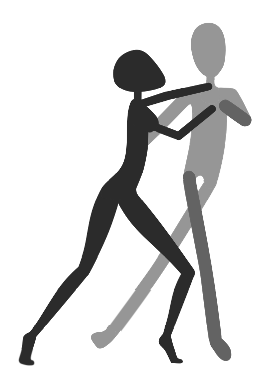
\includegraphics[width=0.49\textwidth]{logos/logo-bw-1}}} % Image background
%\AddToShipoutPictureBG*{\includegraphics[width=\paperwidth,height=\paperheight]{golden-ratio-3}}
%
\noindent\begin{minipage}{\textwidth}
\centering\fontsize{0.032\textheight}{0pt}\selectfont%
\vspace*{0.18\textheight}%
\TextAtTopOfPage%
\vspace*{0.18\textheight}%
\end{minipage}
%
\noindent\begin{minipage}{\textwidth}
\centering%
{\fontsize{0.06\textheight}{0}\selectfont \BookTitle\\[0.02\textheight]}%
{\fontsize{0.05\textheight}{0}\selectfont \BookSubTitle}%
\end{minipage}
\vspace{0.14\textheight}
\begin{center}
    {\fontsize{0.032\textheight}{0pt}\selectfont \BookAuthor}\\[1\baselineskip]
    {\fontsize{0.032\textheight}{0pt}\selectfont \BookEditionLocal}\\[1\baselineskip]
    {\fontsize{0.032\textheight}{0pt}\selectfont \TextAtBottomOfPage}
\end{center}
%
\end{titlepage}
\endgroup
 % titlepage [model-1 ..model-4]

%-------------------------------------------------------------------------------
%   COPYRIGHT PAGE
%-------------------------------------------------------------------------------
%\cleardoublepage

\newpage
\thispagestyle{empty}

\noindent Copyright \copyright\ \BookEditionYear\ \BookAuthor.\ % Copyright notice

\begin{wrapfigure}{l}{0.3\textwidth}
\vspace{-10pt}
\includegraphics[width=0.29\textwidth]{logos/by-nc-nd.png}
\vspace{-10pt}
\end{wrapfigure}
\noindent This work is licensed under the Creative Commons Attribution-NonCommercial-NoDerivatives 4.0 International License.
You may use this file only in accordance with the License. Obtain a copy of the license at:
\url{https://creativecommons.org/licenses/by-nc-nd/4.0/}.\\ % License information

\noindent \textbf{Limitation of Liability and Disclaimer of Warranty:}
This book has been prepared with care and dedication,
with the intent to be useful and informative.
However, the author assumes no responsibility for any inaccuracies or omissions,
nor does he make any warranties of accuracy or completeness.

~

\noindent Be sure to ``download'' the digital version of the book at \BookLinkHomePage.

~

\noindent \textbf{Printed in Brazil -- ISBN:} \BookISBN.\\ % Publisher
\noindent \textbf{First printing:} 2024.\\ % Printing/edition date
\noindent \textbf{Proofreading:} \BookAuthor.\\ % Printing/edition date
\noindent \textbf{Layout:} \BookAuthor.\\ % Printing/edition date
\noindent \textbf{Published:} \BookPublisher.\\ % Publisher
\noindent \textbf{Cover:} \BookAuthor. % Printing/edition date

~


\SetCardColorFrame{white}
\SetBookAuthorLastName{\BookAuthorLastName}
\SetBookAuthorName{\BookAuthorName}
\SetBookAuthorYearBorn{\BookAuthorBorn}
\SetBookTitle{\BookTitle}
\SetBookSubTitle{\BookSubTitle}
\SetBookPublishingPlace{\BookEditionLocal}
\SetBookPublishingEditor{\BookPublisher}
\SetBookPublishingYear{\BookEditionYear}
\SetBookPaperSize{\BookPaperSizeString}
\SetBookHasBibliography{\BookHasBibliography}
\SetBookISBN{\BookISBN}
\SetBookKeyWordA{\BookKeyWordA}
\SetBookKeyWordB{\BookKeyWordB}
\SetBookKeyWordC{\BookKeyWordC}
\SetBookSearchBy{Title}
\SetBookCDD{\BookCDD}
\SetBookCDU{\BookCDU}

~

\begin{center}
\CatalographicCard{12.5cm}
\end{center}




%-------------------------------------------------------------------------------
%   DEDICATORIA
%-------------------------------------------------------------------------------
\cleardoublepage

\null
\vfill
\thispagestyle{empty}



{\normalsize \it \hfill Amicum lege feliciter, vivas, gaudeas, floreas in Deo. \vspace*{4pt}

%\hfill understanding and assistance they have given me. \vspace*{4pt}

\hfill Fernando \vspace*{4pt}}

 

%-------------------------------------------------------------------------------
%   Acknowledgements
%-------------------------------------------------------------------------------
\cleardoublepage
\thispagestyle{empty}


\chapter*{Agradecimentos}

\vfill


{\normalsize \it \hfill Dou muitas graças a Deus \vspace*{4pt}}


~\\

\begin{comment}
{\normalsize \it Dou muitas graças a Estevam Lawrence por me 
ajudar a resolver muitas duvidas sobre definições e uso de termos na teoria musical.
\vspace*{4pt}}
\end{comment}

\begin{comment}
{\normalsize \it Dou muitas graças ao Prof. José Henrique de Souza (Henrique Carioca)
por suas aulas de samba no pê, 
e ter-me ensinado exercícios para o desenvolvimento da consciência corporal.
\vspace*{4pt}}
\end{comment}

\begin{comment}
{\normalsize \it Dou muitas graças ao Prof. Jaime Arôxa por me 
ajudar a resolver algumas duvidas sobre definições e uso de termos na pedagogia para o ensino do samba de gafieira.
\vspace*{4pt}}
\end{comment}

\begin{comment}
{\normalsize \it Dou muitas graças a \textcolor{red}{XXXXXXXXXXX} pela 
suas sugestões e revisão  do capitulo \textcolor{red}{XXXXXXXXXXX}.
\vspace*{4pt}}
\end{comment}


 

%-------------------------------------------------------------------------------
%   PATROCINIO PAGE
%-------------------------------------------------------------------------------
\cleardoublepage

\newpage
\thispagestyle{empty}


\vfill

\begin{center}
\Huge{\textbf{Patrocínio}}
\end{center}

\vfill


\begin{tcolorbox}[colback = colorPatrocinio, colframe = colorPatrocinio]%%
	\sffamily
	\begin{center}					% Minipage Centralizado
	\fboxsep=10pt
	\fbox{ \begin{minipage}[c][]{\textwidth-\fboxsep-\fboxsep}		% Largura

    \hspace{0.5cm}
    Se deseja investir nesta pesquisa, colaborando com o desenvolvimento e crescimento do projeto,
    então convido você a adquirir um exemplar deste livro. 
    Para ver uma lista com indicações sobre onde comprar uma versão impressa ou digital desta obra, dirija-se a: 
    \begin{itemize}
    \item \ImprimirLinkCompraLivroImpresso 
    \item \ImprimirLinkCompraLivroDigital \\ 
    \end{itemize}


    \hspace{0.5cm}
    Também pode colaborar com dinheiro em efetivo, desde 15 reais,  
    mediante PIX pelo seguinte código QR:

    %% 00020126580014BR.GOV.BCB.PIX0136260e95c5-b78b-4720-baa5-679326da195c520400005303986540515.005802BR5923Fernando Pujaico Rivera6009SAO PAULO61080540900062240520mZOkk6HGwQrlucfqh55763046D39
    \begin{center}
    \ImprimirLinkMetodoPagoA 
    \end{center}


    \hspace{0.5cm}
    Se já colaborou com esta pesquisa, e se assim o desejar, 
    sinta-se livre de me mandar um correio eletrônico no endereço
    \ImprimirEmail, 
    sugerindo a abordagem de um novo assunto ou o aprofundamento em outro.
    Se seu pedido está dentro das minhas capacidades, 
    este será agregado sem falta na seguinte edição do livro.

    \begin{flushright}
    \myauthor ~
    \end{flushright}

	\end{minipage}}
	\end{center}
\end{tcolorbox}%%

\vfill



%-------------------------------------------------------------------------------
%   PATROCINIO PAGE
%-------------------------------------------------------------------------------

\cleardoublepage % Forces the first chapter to start on an odd page so it's on the right
\pagestyle{fancy} % Print headers again

\chapter*{Prologue}
\addcontentsline{toc}{chapter}{Prologue} %% Sale en la pagina contents

Science is a journey of curiosity, observation, and understanding. 
Through careful analysis and persistent inquiry, 
we uncover patterns in nature and formulate principles that help us explain the world around us.

This book is the result of dedicated research and aims to contribute to the growing body of scientific knowledge. 
It is written with the hope that it may inspire further exploration, critical thinking, and informed discussion.

Let this be an invitation to think deeply, question boldly, and learn continually.



%-------------------------------------------------------------------------------
%   TABLE OF CONTENTS
%-------------------------------------------------------------------------------
\clearpage
\pagestyle{fancy} %\pagestyle{empty} % No headers %\pagestyle{fancy} % Print headers again
\tableofcontents % Print the table of contents itself

%-------------------------------------------------------------------------------
%   TABLE OF DATAS % theorems, definitions, examples, etc.
%-------------------------------------------------------------------------------


%----------------------------------------------------------------------------------------
%	TABLE OF LISTAS
%----------------------------------------------------------------------------------------
\chapter*{Listas de dados}
\addcontentsline{toc}{chapter}{Listas de dados} %% Sale en la pagina contents


%----------------------------------------------------------------------------------------
%    LISTA DE DEFINICIONES
%----------------------------------------------------------------------------------------
\phantomsection
\addcontentsline{toc}{section}{Lista de definições} %% Sale en la pagina contents
\tcblistof[\section*]{MisDefinicoes}{Lista de definições}
%----------------------------------------------------------------------------------------
%    LISTA DE TEOREMAS
%----------------------------------------------------------------------------------------
\phantomsection
\addcontentsline{toc}{section}{Lista de teoremas} %% Sale en la pagina contents
\tcblistof[\section*]{MisTheorem}{Lista de teoremas}
%----------------------------------------------------------------------------------------
%    LISTA DE NOTACIONES
%----------------------------------------------------------------------------------------
\phantomsection
\addcontentsline{toc}{section}{Lista de notações} %% Sale en la pagina contents
\tcblistof[\section*]{MisNotation}{Lista de notações}
%----------------------------------------------------------------------------------------
%    LISTA DE EXEMPLOS
%----------------------------------------------------------------------------------------
\phantomsection
\addcontentsline{toc}{section}{Lista de exemplos} %% Sale en la pagina contents
\tcblistof[\section*]{MisExample}{Lista de exemplos}
%----------------------------------------------------------------------------------------
%    LISTA DE EXERCICIOS
%----------------------------------------------------------------------------------------
\phantomsection
\addcontentsline{toc}{section}{Lista de exercicíos} %% Sale en la pagina contents
\tcblistof[\section*]{MisExercise}{Lista de exercicíos}

%----------------------------------------------------------------------------------------
%    LISTA DE INFORMACOES
%----------------------------------------------------------------------------------------
\phantomsection
\addcontentsline{toc}{section}{Lista de informações} %% Sale en la pagina contents
\tcblistof[\section*]{MisInformacoes}{Lista de informações}
%----------------------------------------------------------------------------------------
%    LISTA DE ELABORACIONES
%----------------------------------------------------------------------------------------
% temas sueltos que sao elaborado para anhadir riqueza a experiencia de leitura
\phantomsection
\addcontentsline{toc}{section}{Lista de elaborações} %% Sale en la pagina contents
\tcblistof[\section*]{MisElaboraciones}{Lista de elaborações}

%----------------------------------------------------------------------------------------
%    LISTA DE FRASES
%----------------------------------------------------------------------------------------
\phantomsection
\addcontentsline{toc}{section}{Lista de frases} %% Sale en la pagina contents
\tcblistof[\section*]{MisFrases}{Lista de frases}




%-------------------------------------------------------------------------------
\cleardoublepage % Forces the first chapter to start on an odd page so it's on the right
\pagestyle{fancy} % Print headers again


%-------------------------------------------------------------------------------
%   PART
%-------------------------------------------------------------------------------
\part{Sample of text}

\chapter{Text Chapter: Full Connected Neural Network}

%-------------------------------------------------------------------------------
\section{Paragraphs of Text}\index{Paragraphs of Text}

\lipsum[1][1-3] 

\begin{informationbox}{Título A}
\lipsum[1][1-3] 
\end{informationbox}

\lipsum[1][1-3]

\HTextRule{Text}

\begin{frasebox}{Frase title A}{Autor}
\lipsum[1][1-3] 
\end{frasebox}

\begin{frasebox}{Frase title B}{Autor}
\lipsum[1][1-3] 
\end{frasebox}

\lipsum[1][1-3] 

\begin{citationbox}
\lipsum[1][1-3] 
\end{citationbox}

%-------------------------------------------------------------------------------
\section{Citation}\index{Citation}

This statement requires citation \cite{book_key}; this one is more specific \cite[122]{article_key}.

\lipsum[1] % 

\begin{informationbox}{Título B}
\lipsum[1][1-3]\footnote{Simple footnote example.}
\end{informationbox}

\lipsum[1] % 

\begin{elaborationbox}{Título C}
\lipsum[1][1-3] 
\end{elaborationbox}

%-------------------------------------------------------------------------------
\section{Lists}\index{Lists}

\lipsum[1][1-3]\footnote{Footnote example...}.

\subsection{Numbered List}\index{Lists!Numbered List}

\begin{enumerate}
\item \lipsum[1][1-3].
\item \lipsum[1][1-3].
\item \lipsum[1][1-3].
\end{enumerate}

\subsection{Bullet Points}\index{Lists!Bullet Points}

\begin{itemize}
\item \lipsum[1][1-3].
\item \lipsum[1][1-3].
\item \lipsum[1][1-3].
\end{itemize}

\subsection{Descriptions and Definitions}\index{Lists!Descriptions and Definitions}

\begin{description}
\item[Name] \lipsum[1][1-3].
\item[Word] \lipsum[1][1-3].
\item[Comment] \lipsum[1][1-3].
\end{description}



%-------------------------------------------------------------------------------
%   PART
%-------------------------------------------------------------------------------
\part{Enviroments}

\chapter{In-text Elements}

\section{Boxs}\index{Boxs}

This is an example of use theorem. 
We can reference the Theorem \ref{theo:A}, \ref{theo:B}, \ref{theo:C}, \ref{theo:D} and \ref{theo:E}.

%-------------------------------------------------------------------------------
\subsection{Theorems}\index{Theorems!Several Equations}

This is an example of theorem.
\begin{verbatim}
\begin{theorem}[Name of the theorem]
\label{theo:A}
\lipsum[1][1-3]
\begin{equation}
x^2+e^{-\frac{x^2}{2}}=1
\end{equation}
\end{theorem}
\end{verbatim}

The last code generates the next theorem.
\begin{theorem}[Name of the theorem]
\label{theo:A}
\lipsum[1][1-3]
\begin{equation}
x^2+e^{-\frac{x^2}{2}}=1
\end{equation}
\end{theorem}

This is an example of theorem proof.
\begin{verbatim}
\begin{proofraw}[Relative to Teorema \ref{theo:A}]
\lipsum[1][1-3]
\begin{equation}
x^2+e^{-\frac{x^2}{2}}=1
\end{equation}
\end{proofraw}
\end{verbatim}
The last code gnerates the next proof.
\begin{proofraw}[Relative to Teorema \ref{theo:A}]
\lipsum[1][1-3]
\begin{equation}
x^2+e^{-\frac{x^2}{2}}=1
\end{equation}
\end{proofraw}

\subsection{Exercises}\index{Exercises!Single Line}
\lipsum[1][1-3]

\begin{verbatim}
\begin{exercise}[Exercise name]
\lipsum[1][1-3]
\begin{equation}
x^2+e^{-\frac{x^2}{2}}=1
\end{equation}
\end{exercise}
\end{verbatim}
\begin{exercise}[Exercise name]
\lipsum[1][1-3]
\begin{equation}
x^2+e^{-\frac{x^2}{2}}=1
\end{equation}
\end{exercise}

\begin{verbatim}
\begin{exercise}[Exercise name A0]
\label{ex:A0}
\lipsum[1][1-3]
\begin{equation}
x^2+e^{-\frac{x^2}{2}}=1
\end{equation}
\end{exercise}
\end{verbatim}
\begin{exercise}[Exercise name A0]
\label{ex:A0}
\lipsum[1][1-3]
\begin{equation}
x^2+e^{-\frac{x^2}{2}}=1
\end{equation}
\end{exercise}

\begin{verbatim}
\begin{theorem}
\label{theo:B}
\lipsum[1][1-3]
\end{theorem}
\end{verbatim}
\begin{theorem}
\label{theo:B}
\lipsum[1][1-3]
\end{theorem}

%-------------------------------------------------------------------------------
\section{Examples}\index{Examples}
\lipsum[1][1-3]
See Example \ref{ex:A0}

\begin{verbatim}
\begin{example}[Example name]
\label{ex:A0:b}
\lipsum[1][1-3]
\begin{equation}
x^2+e^{-\frac{x^2}{2}}=1
\end{equation}
\end{example}
\end{verbatim}
\begin{example}[Example name]
\label{ex:A0:b}
\lipsum[1][1-3]
\begin{equation}
x^2+e^{-\frac{x^2}{2}}=1
\end{equation}
\end{example}

\begin{verbatim}
\begin{theorem}
\label{theo:C}
\lipsum[1][1-3]
\end{theorem}
\end{verbatim}
\begin{theorem}
\label{theo:C}
\lipsum[1][1-3]
\end{theorem}

\begin{verbatim}
\begin{theorem}
\label{theo:D}
\lipsum[1][1-3]
\end{theorem}
\end{verbatim}
\begin{theorem}
\label{theo:D}
\lipsum[1][1-3]
\end{theorem}


%-------------------------------------------------------------------------------
\section{Definitions}\index{Definitions}

Definition \ref{def:A0},
\begin{verbatim}
\begin{definition}[Definition name]
\label{def:A0}
\lipsum[1][1-3]
\begin{equation}
x^2+e^{-\frac{x^2}{2}}=1
\end{equation}
\end{definition}
\end{verbatim}
\begin{definition}[Definition name]
\label{def:A0}
\lipsum[1][1-3]
\begin{equation}
x^2+e^{-\frac{x^2}{2}}=1
\end{equation}
\end{definition}

\begin{verbatim}
\begin{theorem}[Theorem name]
\label{theo:E}
\lipsum[1][1-3]
\begin{equation}
x^2+e^{-\frac{x^2}{2}}=1
\end{equation}
\end{theorem}
\end{verbatim}
\begin{theorem}[Theorem name]
\label{theo:E}
\lipsum[1][1-3]
\begin{equation}
x^2+e^{-\frac{x^2}{2}}=1
\end{equation}
\end{theorem}

\begin{verbatim}
\begin{exercise}[Exercise name A]
\label{exer:A}
\lipsum[1][1-3]
\begin{equation}
x^2+e^{-\frac{x^2}{2}}=1
\end{equation}
\end{exercise}
\end{verbatim}
\begin{exercise}[Exercise name A]
\label{exer:A}
\lipsum[1][1-3]
\begin{equation}
x^2+e^{-\frac{x^2}{2}}=1
\end{equation}
\end{exercise}

\begin{verbatim}
\begin{exercise}[Exercise name]
\lipsum[1][1-3]
\begin{equation}
x^2+e^{-\frac{x^2}{2}}=1
\end{equation}
\end{exercise}
\end{verbatim}
\begin{exercise}[Exercise name]
\lipsum[1][1-3]
\begin{equation}
x^2+e^{-\frac{x^2}{2}}=1
\end{equation}
\end{exercise}

\begin{verbatim}
\begin{exercise}[Exercise name B]
\label{exer:B}
\lipsum[1][1-3]
\begin{equation}
x^2+e^{-\frac{x^2}{2}}=1
\end{equation}
\end{exercise}
\end{verbatim}
\begin{exercise}[Exercise name B]
\label{exer:B}
\lipsum[1][1-3]
\begin{equation}
x^2+e^{-\frac{x^2}{2}}=1
\end{equation}
\end{exercise}


Exer \ref{ex:A0}, \ref{exer:A} e \ref{exer:B}.

%-------------------------------------------------------------------------------
\section{Notations}\index{Notations}

Notations \ref{not:A}, \ref{not:B}, \ref{not:C} e \ref{not:D}.

\begin{verbatim}
\begin{notation}
\label{not:A}
\lipsum[1][1-3]
\begin{equation}
x^2+e^{-\frac{x^2}{2}}=1
\end{equation}
\end{notation}
\end{verbatim}
\begin{notation}
\label{not:A}
\lipsum[1][1-3]
\begin{equation}
x^2+e^{-\frac{x^2}{2}}=1
\end{equation}
\end{notation}

\begin{verbatim}
\begin{notation}[Notation name title very large]
\label{not:B}
\lipsum[1][1-3]
\begin{equation}
x^2+e^{-\frac{x^2}{2}}=1
\end{equation}
\end{notation}
\end{verbatim}
\begin{notation}[Notation name title very large]
\label{not:B}
\lipsum[1][1-3]
\begin{equation}
x^2+e^{-\frac{x^2}{2}}=1
\end{equation}
\end{notation}

\begin{verbatim}
\begin{notation}
\label{not:C}
\lipsum[1][1-3]
\begin{equation}
x^2+e^{-\frac{x^2}{2}}=1
\end{equation}
\end{notation}
\end{verbatim}
\begin{notation}
\label{not:C}
\lipsum[1][1-3]
\begin{equation}
x^2+e^{-\frac{x^2}{2}}=1
\end{equation}
\end{notation}

\begin{verbatim}
\begin{notation}[Notation title]
\label{not:D}
\lipsum[1][1-3]
\end{notation}
\end{verbatim}
\begin{notation}[Notation title]
\label{not:D}
\lipsum[1][1-3]
\end{notation}

%------------------------------------------------

\section{Equationbox}\index{Equationbox}

\begin{verbatim}
\begin{equationbox}
\begin{equation}
x^2+e^{-\frac{x^2}{2}}=1
\end{equation}
\end{equationbox}
\end{verbatim}
\begin{equationbox}
\begin{equation}
x^2+e^{-\frac{x^2}{2}}=1
\end{equation}
\end{equationbox}


\section{Phrasebox}\index{Phrasebox}

\begin{verbatim}
\begin{phrasebox}{Frase title}{Fernando P. R.}
\lipsum[1][1-3]
\end{phrasebox}
\end{verbatim}
\begin{phrasebox}{Frase title}{Fernando P. R.}
\lipsum[1][1-3]
\end{phrasebox}
%------------------------------------------------

\section{Attentionbox}\index{Attentionbox}

\lipsum[1][1-3]

\begin{verbatim}
\begin{attentionbox}
\lipsum[1][1-3] 
\end{attentionbox}
\end{verbatim}
\begin{attentionbox}
\lipsum[1][1-3] 
\end{attentionbox}


%------------------------------------------------

\section{Informationbox}\index{Informationbox}

\lipsum[1][1-3]

\begin{verbatim}
\begin{informationbox}[Título A]
\lipsum[1][1-3]
\end{informationbox}
\end{verbatim}
\begin{informationbox}[Título A]
\lipsum[1][1-3]
\end{informationbox}

%------------------------------------------------

\section{Elaborationbox}\index{Elaborationbox}

\lipsum[1][1-3]

\begin{verbatim}
\begin{elaborationbox}[Title of elaborationbox]
\lipsum[1][1-3]
\end{elaborationbox}
\end{verbatim}
\begin{elaborationbox}[Title of elaborationbox]
\lipsum[1][1-3]
\end{elaborationbox}

\lipsum[1][1-3]
\begin{verbatim}
\begin{elaborationbox}
\lipsum[1][1-3]
\end{elaborationbox}
\end{verbatim}
\begin{elaborationbox}
\lipsum[1][1-3]
\end{elaborationbox}

%------------------------------------------------

\section{Bulletjournalitem}\index{Bulletjournalitem}

\lipsum[1][1-3]

\begin{verbatim}
\begin{bulletjournalitem}
\tcbitem \lipsum[1][1-3]
\tcbitem \lipsum[1][2-4]
\tcbitem \lipsum[1][3-5]
\end{bulletjournalitem}
\end{verbatim}

\begin{bulletjournalitem}
\tcbitem \lipsum[1][1-3]
\tcbitem \lipsum[1][2-4]
\tcbitem \lipsum[1][3-5]
\end{bulletjournalitem}

%------------------------------------------------

\section{Bulletjournalpicture}\index{Bulletjournalpicture}

\lipsum[1][1-3]

\begin{verbatim}
\begin{bulletjournalpicture}[black]
\tcbitem \lipsum[1][1-3]
\tcbitem \lipsum[1][2-4]
\tcbitem \lipsum[1][3-5]
\end{bulletjournalpicture}
\end{verbatim}

\begin{bulletjournalpicture}[black]
\tcbitem \lipsum[1][1-3]
\tcbitem \lipsum[1][2-4]
\tcbitem \lipsum[1][3-5]
\end{bulletjournalpicture}
%------------------------------------------------

\section{Bulletjournalarrow}\index{Bulletjournalarrow}

\lipsum[1][1-3]

\begin{verbatim}
\begin{bulletjournalarrow}[black]
\tcbitem First line of text.
\tcbitem Second line of text.
\end{bulletjournalarrow}
\end{verbatim}
\begin{bulletjournalarrow}[black]
\tcbitem First line of text.
\tcbitem Second line of text.
\end{bulletjournalarrow}




%------------------------------------------------

\section{Bulletjournalround}\index{Bulletjournalround}

\begin{verbatim}
\begin{bulletjournalround}[colorNotation]
\tcbitem First line of text.
\tcbitem Second line of text.
\end{bulletjournalround}
\end{verbatim}
\begin{bulletjournalround}[colorNotation]
\tcbitem First line of text.
\tcbitem Second line of text.
\end{bulletjournalround}


\lipsum[1][1-3]

\begin{verbatim}
\begin{notation}[Notation name title very large]
Text before bulletjournalround enviroment.
\begin{bulletjournalround}[colorNotation]
\tcbitem First line of text.
\tcbitem Second line of text.
\end{bulletjournalround}
Text out of bulletjournalround enviroment.
\end{notation}
\end{verbatim}
\begin{notation}[Notation name title very large]
Text before bulletjournalround enviroment.
\begin{bulletjournalround}[colorNotation]
\tcbitem First line of text.
\tcbitem Second line of text.
\end{bulletjournalround}
Text out of bulletjournalround enviroment.
\end{notation}

%------------------------------------------------

\section{Notebox}\index{Notebox}

\begin{verbatim}
\begin{notebox}
\lipsum[1][1-3]
\end{notebox}
\end{verbatim}
\begin{notebox}
\lipsum[1][1-3]
\end{notebox}



\chapter{Presenting Information}

\lipsum[1] 
%------------------------------------------------
\section{Table}\index{Table}
\lipsum[1] 
\lipsum[1][1-3]
\begin{highlightbox}
\begin{verbatim}
\begin{table}[h]
\centering
\begin{tabular}{l l l}
\toprule
\textbf{Treat.} & 
\textbf{Resp. 1} & 
\textbf{Resp. 2}\\
\midrule
Treatment 1 & 0.0003262 & 0.562 \\
Treatment 2 & 0.0015681 & 0.910 \\
Treatment 3 & 0.0009271 & 0.296 \\
\bottomrule
\end{tabular}
\caption{Table caption}
\end{table}
\end{verbatim}
\end{highlightbox}
\begin{table}[h]
\centering
\begin{tabular}{l l l}
\toprule
\textbf{Treat.} & \textbf{Resp. 1} & \textbf{Resp. 2}\\
\midrule
Treatment 1 & 0.0003262 & 0.562 \\
Treatment 2 & 0.0015681 & 0.910 \\
Treatment 3 & 0.0009271 & 0.296 \\
\bottomrule
\end{tabular}
\caption{Table caption}
\end{table}

%------------------------------------------------
\section{Figure}\index{Figure}

\lipsum[1] 

\begin{highlightbox}
\begin{verbatim}
\begin{figure}[h]
\centering
\includegraphics[width=0.3\textwidth]
{placeholder.jpg}
\caption{Figure caption}
\end{figure}
\end{verbatim}
\end{highlightbox}
\begin{figure}[h]
\centering\includegraphics[width=0.3\textwidth]{placeholder.jpg}
\caption{Figure caption}
\end{figure}

\begin{attentionbox}
Search image files in directory: ./pictures\\
\end{attentionbox}



%-------------------------------------------------------------------------------
%   PART
%-------------------------------------------------------------------------------
\part{Macros}



%----------------------------------------------------------------------------------------
%	CHAPTER 4
%----------------------------------------------------------------------------------------

\chapter{Macros}



\newcommand{\EXAMPLEOFMATHMACRO}[1]{%
\begin{highlightbox}%
\texttt{\detokenize{\begin{equation}}}\\
\texttt{\detokenize{#1}}\\
\texttt{\detokenize{\end{equation}}}
\end{highlightbox}%
\begin{equation}
#1
\end{equation}\\
}




\section{File math-macros.tex}

\EXAMPLEOFMATHMACRO{\FuncOf{f}{x}}


\EXAMPLEOFMATHMACRO{\MinOf{x}{f(x)}}

\EXAMPLEOFMATHMACRO{\ArgMin{x}{f(x)}}

\EXAMPLEOFMATHMACRO{\ArgMinDef{x}{f}}

\EXAMPLEOFMATHMACRO{\EigenSet{A}{v}{\lambda}}

\EXAMPLEOFMATHMACRO{\InnerProd{x}{y}}

\EXAMPLEOFMATHMACRO{\Norm{x}}

\EXAMPLEOFMATHMACRO{\Cardinality{x}}

\EXAMPLEOFMATHMACRO{\DiagFunc{x}}

\EXAMPLEOFMATHMACRO{\Vector{x}}

\EXAMPLEOFMATHMACRO{\Matrix{x}}

\EXAMPLEOFMATHMACRO{\DtVector{x}}

\EXAMPLEOFMATHMACRO{\DDtVector{x}}

\EXAMPLEOFMATHMACRO{\DtMatrix{x}}

\EXAMPLEOFMATHMACRO{\DDtMatrix{x}}

\EXAMPLEOFMATHMACRO{\DPartial{y}{x}}

\EXAMPLEOFMATHMACRO{\DDPartial{y}{x}}

\EXAMPLEOFMATHMACRO{\DDPartialXY{z}{x}{y}}






%-------------------------------------------------------------------------------
%   Apendice
%-------------------------------------------------------------------------------
%\part{Apendice}



%-------------------------------------------------------------------------------
%   PART
%-------------------------------------------------------------------------------
\part{Referencias}

%-------------------------------------------------------------------------------
%   BIBLIOGRAPHY
%-------------------------------------------------------------------------------
\chapter*{Bibliografia}
\addcontentsline{toc}{chapter}{Bibliografia} %% Sale en la pagina part
\printbibliography[heading=bibempty]

%-------------------------------------------------------------------------------
%   INDEX
%-------------------------------------------------------------------------------
\cleardoublepage
\phantomsection
\setlength{\columnsep}{0.75cm}
\addcontentsline{toc}{chapter}{Índice} %% Sale en la pagina part
\printindex

%-------------------------------------------------------------------------------

%-------------------------------------------------------------------------------
%   COLOFÃO
%-------------------------------------------------------------------------------
\cleardoublepage

\null
\vfill
\newpage

\null
\vfill
\thispagestyle{empty}



{\normalsize \it This book was produced by \BookAuthor, edited and designed using \LaTeX,
with a font of \fprshowfont,
to be printed on paper size \BookPaperSizeString. Edition created on \BookEditionDate.
\vspace*{4pt}}








\end{document}
